    \documentclass[12pt]{article}
    \usepackage{fancyhdr, amsmath, amsthm, amssymb, mathtools, lastpage,
    hyperref, enumerate, graphicx, setspace, wasysym, upgreek, listings}
    \usepackage{geometry}
    \newcommand{\scinot}[2]{#1\times10^{#2}}
    \newcommand{\bra}[1]{\left<#1\right|}
    \newcommand{\ket}[1]{\left|#1\right>}
    \newcommand{\dotp}[2]{\left<#1\,\middle|\,#2\right>}
    \newcommand{\rd}[2]{\frac{\mathrm{d}#1}{\mathrm{d}#2}}
    \newcommand{\pd}[2]{\frac{\partial#1}{\partial#2}}
    \newcommand{\rtd}[2]{\frac{\mathrm{d}^2#1}{\mathrm{d}#2^2}}
    \newcommand{\ptd}[2]{\frac{\partial^2 #1}{\partial#2^2}}
    \newcommand{\norm}[1]{\left|\left|#1\right|\right|}
    \newcommand{\abs}[1]{\left|#1\right|}
    \newcommand{\pvec}[1]{\vec{#1}^{\,\prime}}
    \newcommand{\tensor}[1]{\overleftrightarrow{#1}}
    \let\Re\undefined
    \let\Im\undefined
    \newcommand{\ang}[0]{\text{\AA}}
    \newcommand{\mum}[0]{\upmu \mathrm{m}}
    \DeclareMathOperator{\Re}{Re}
    \DeclareMathOperator{\Im}{Im}
    \DeclareMathOperator{\Log}{Log}
    \DeclareMathOperator{\Arg}{Arg}
    \DeclareMathOperator{\Tr}{Tr}
    \DeclareMathOperator{\E}{E}
    \DeclareMathOperator{\Var}{Var}
    \DeclareMathOperator*{\argmin}{argmin}
    \DeclareMathOperator*{\argmax}{argmax}
    \DeclareMathOperator{\sgn}{sgn}
    \newcommand{\expvalue}[1]{\left<#1\right>}
    \usepackage[labelfont=bf, font=scriptsize]{caption}\usepackage{tikz}
    \usepackage[font=scriptsize]{subcaption}
    \everymath{\displaystyle}
    \lstset{basicstyle=\ttfamily\footnotesize,frame=single,numbers=left}

\tikzstyle{circ} = [draw, circle, fill=white, node distance=3cm, minimum
height=2em]

\begin{document}

\onehalfspacing

\pagestyle{fancy}
\rhead{Yubo Su --- Independent Study: Ph161}
\cfoot{\thepage/\pageref{LastPage}}

\tableofcontents
\clearpage

\section{Key Concepts}

Note that Poincar\'e sections allow us to turn flows into maps!

We begin the class by exploring various chaotic maps, but a few
characterizations that we've learned include:
\begin{description}
    \item[Power Spectrum] Typically periodic trajectories have very sharp peaks
        in their power spectrum, and quasi-periodic trajectories simply have
        peaks at frequencies that do not share a common factor. Chaotic
        trajectories have a broad power spectrum.

    \item[Lyapunov Exponents] Lyapunov exponents let us quantify, for a given
        initial condition, how much phase space is expanding at that point. A
        positive Lyapunov Exponent implies nearby points diverge exponentially
        and are indicative of chaotic dynamics.

    \item[Entropy] Kolmogorov Entropy is a measure of how many partitions a
        single partitioning in a partition maps to under a map. In non-chaotic
        dynamics, we would expect certain partitions to map strictly within
        themselves, but if this mixing is always positive, then the Kolmogorov
        Entropy is positive and suggests chaotic dynamics.

    \item[Period Doubling Route to Chaos] Some dynamical systems parameterized
        by some $\alpha$ will exhibit period doubling bifurcations as $\alpha$
        is increased. If these bifurcations happen for increasingly small
        changes in $\alpha$, its possible for some finite $\alpha$ that the
        system enters chaos i.e.\ infinite period.

    \item[Renormalization Group] In large broad strokes, renormalization in
        chaos is the procedure $T[f(x)] = -\alpha f(f(-x/\alpha))$, whereby we
        rescale coordinates. In period doubling cascades, renormalization shows
        us given a rather general set of assumptions how period doubling comes
        about.

    \item[Chaos in non-attracting sets] Chaos can also be described in terms of
        symbolic dynamics, where we construct some mapping from phase space to a
        discrete sequence of variables e.g.\ $0$s and $1$s. We then state that a
        system is chaotic if for every such sequence we can find a set of
        initial conditions to produce this sequence.
\end{description}

\section{Lorenz Model}

The Lorenz Model arises as an approximation to atmospheric flow, starting with
the description of the simplest mode of a convection zone and dropping terms
that represent higher harmonics. This gives the following system of equations
\begin{align}
    \dot{X} &= -\sigma(X - Y) \nonumber\\
    \dot{Y} &= rX - Y - XZ \nonumber\\
    \dot{Z} &= b(XY - Z)
\end{align}
with parameters canonically set at $\sigma = 10, b = 8/3, r =27 > 1$ (note that
$\sigma$ is 0.7 for an ideal gas, 1--4 for water and $>10$ for oils). Note that
the equations are dissipative, i.e.\ volumes in phase space shrink in dynamics.
Note also that they are \emph{autonomous} in that there is no explicit time
dependence on the right hand side, a convenient property.

It turns out that the solutions to this system are chaotic, or in Lorenz's
original terms ``aperiodic.'' We do many demonstrations that are no longer
accessible, including \emph{strange attractors, Poincar\'e section} and
\emph{1D maps}.

The last is going to be covered in a later lecture, but in case I'm interested
in simulating the former two, I look them up here (the website has discussions
of these with the applets absent):
\begin{itemize}
    \item Poincar\'e section examines the intersection of an orbit with a
        particular plane in phase space, e.g.\ $Z=31$ is a common one. So we
        just simulate and examine every time that $Z=31$ is crossed, exactly
        what $(X,Y)$ are.
    \item Strange attractors are subsets of phase space with fractional
        dimension (fractals) that orbits at long times lie in.
\end{itemize}

\clearpage

\section{Pendula}

\subsection{Ideal Pendulum}

The ideal pendulum is given by EOM $\rtd{\theta}{t} + \frac{g\sin\theta}{l} =
0$. We can plot phase space $(\theta, \omega = \dot{\theta})$ for solution
trajectories. There are a few features of interest
\begin{itemize}
    \item Fixed points --- Two types, elliptic (stable but not asymptotically
        stable) and hyperbolic (unstable)
    \item Limit Cycles --- Solution trajectories.
    \item Homoclinic orbits --- Trajectories that connect the same hyperbolic
        fixed point. Heteroclinic orbits connect two different hyperbolic fixed
        points.
\end{itemize}

We can write down the Hamiltonian for this system $H = \frac{J^2}{2I} +
Mgl(1-\cos\theta)$. The importance of being able to do is that phase space
volume is preserved. What do we mean by this? Well, consider Hamilton's
canonical equations
\begin{align}
    \dot{\theta} = \pd{H}{J} &= \frac{J}{I} \nonumber\\
    \dot{J} = -\pd{H}{\theta} &= -Mgl\sin\theta
\end{align}
and if we define some phase space velocity $\vec{V} = \left( \dot{\theta},
\dot{J} \right)$ we can verify that $\nabla \cdot \vec{V} = 0$. In other words,
no attractors in phase space can exist for a Hamiltonian system.

\subsection{Dissipative Pendulum}

New EOM is $\rtd{\theta}{t} + \eta \rd{\theta}{t} + \frac{g}{l}\sin\theta = 0$.
This creates a fixed point at $(0,0)$, asymptotically stable (``linearly
stable'' is his terminology), and $(\pi,0)$ is suddenly linearly unstable, in
that we will exponentially deviate from the point (before, we still
periodically returned).

\subsection{Driving + damping}

Let's drive the pendulum and rescale variables to $\rtd{\theta}{t} + \gamma
\rd{\theta}{t} + \sin\theta = g\cos(\omega_D t)$. Under small angle
approximation (small amplitude of solution and driving), we know how to solve
this. What about with larger driving amplitudes though?

To handle this, we wish to solve numerically, which is much easier with an
autonomous system than with an explicit time dependence. Thus, we introduce
$\dot{\theta}_D = \omega_D$ and suddenly we can write
\begin{align}
    \dot{\theta} &= \omega \nonumber\\
    \dot{\omega} &= -\gamma \omega - \sin\theta + g\cos(\theta_D) \nonumber\\
    \dot{\theta}_D &= \omega_D
\end{align}

This is a handy trick to get an autonomous system at the expense of an
additional equation in the system of ODEs. We might also suspect that the
behavior of the system changes when we get an extra dimension of phase space.

Well, let's start by observing that $\vec{\nabla} \cdot \vec{v} = -\gamma$ so
phase space volumes contract. This might naively lead us to conclude that any
volume of initial conditions must contract to a point, but we mustn't be hasty;
the Lorenz model also has contracting phase space volumes. Instead, we know
that we might approach a limit cycle in a way such that while the overall phase
space contracts, the space might ``stretch'' along some dimensions and contract
in others such that chaotic dynamics are observed! The demonstrations
illustrating this are broken, but we will definitely simulate this.

\clearpage

\section{Nonlinear Oscillators}

\subsection{Van der Pol Oscillator}

Consider the following model of a harmonic oscillator to include a non-linear
damping. Damping is negative at small amplitudes to model local instability,
but is positive for larger amplitudes; we thus expect the system to have some
limit cycles where the average damping vanishes. The EOM is
\begin{align}
    \ddot{x} - \gamma(1-x^2)\dot{x} + x &= g\cos(\omega_D t)
\end{align}

\subsubsection{Small $\gamma$, secular perturbation}

Let's first look at oscillations with no driving, $g=0$. We return to the
second order EOM for this. The natural starting point is to also examine for
small $\gamma$ and try Lindstedt-Poincar\'e perturbation theory (also called
secular perturbation theory) on
\begin{align}
    \ddot{x} + x &= \gamma(1-x^2)\dot{x}
\end{align}

We begin with the $\gamma=0$ solution, which is just $x(t) = ae^{it + \phi}$.
Then, by secular perturbation theory\footnote{We learned as
\emph{Lindstedt-Poincar\'e} in 106, but this seems to differ slightly; instead
of setting up this slowly varying timescale as below, we tend to set $s = \omega
t$ and expand $\omega = 1 + \epsilon \omega_1 +\dots$.}, when $\gamma \neq 0$,
we can substitute $x(t) = A(t)\cos(t) + \gamma x_1 +\dots$ and also expect
$A(t)$ to be some slow-varying function such that
$\frac{\mathrm{d}^nA(t)}{\mathrm{d}t^n} \sim \gamma^n$ (this is introducing a
second slow time scale, characteristic of secular perturbation theory
apparently) and collect $O(\gamma^1)$ terms in the ODE to obtain
\begin{align}
    \rtd{}{t}\left[ A\cos(t) + \gamma x_1 \right] + A\cos(t) + \gamma x_1 &=
    \gamma(1 - A^2\cos^2(t))\rd{}{t}(A\cos(t)) \nonumber\\
    - 2\sin(t)\rd{A}{t} + \gamma\rtd{x_1}{t} + \gamma x_1 &= -\gamma A\sin(t) +
    \gamma A^3\underbrace{\cos^2(t)\sin(t)}_{\frac{\sin(t)}{4} +
    \frac{\sin(3t)}{4}} \nonumber\\
    \gamma\left(\rtd{x_1}{t} + x_1\right) &= -\gamma A\sin(t) + \gamma
    A^3\frac{\sin(t)}{4} + 2\sin(t)\rd{A}{t} + O(\sin(3t))
\end{align}
where we don't care about the $\sin(3t)$ term since it doesn't drive $x_1$ on
resonance. On the other hand, we require the remaining term vanish, which
implies that
\begin{align}
    2\rd{A}{t} = \gamma A - \frac{\gamma A^3}{4} = \gamma \frac{A(4 - A^2)}{4}
\end{align}
off of which we can read that any initial $A > 0$ tends to grow until $A = 2$,
asymptoting at $x(t) = 2\cos(t)$.

\subsubsection{Large $\gamma$}

For large $\gamma$, let's stick to driving $g=0$ and go to a slightly
unconventional choice of phase space variables, namely
\begin{align}
    \dot{y} &= \ddot{x} - \gamma(1-x^2)\dot{x} = -x\\
    \dot{x} &= y + \gamma\left( x - \frac{x^3}{3} \right)
\end{align}

We then rescle $y \to \gamma Y, t \to \gamma T, x \to X$ and introduce $\eta =
\gamma^{-2}$ and obtain
\begin{align}
    \eta \rd{X}{T} &= Y + \left( X - \frac{X^3}{3} \right)\\
    \rd{Y}{T} &= -X
\end{align}
and for large $\gamma$ we now have small $\eta$. We first find that $\eta = 0$
is inconsistent; the first equation reduces to $Y = -\left( X - \frac{X^3}{3}
\right)$, predicting a minimum of $Y = -\frac{2}{3}$ while the latter suggests
$Y \to 0$ strictly decreasing-ly, contradictory. However, we can still analyze
qualitatively what happens for small $\eta$, an orbit that comprises two pieces
\begin{itemize}
    \item $Y + \left( X - \frac{X^3}{3} \right)$ is small, so $Y \simeq
        \frac{X^3}{3} - X$ and $Y, X$ change on timescales $O(1)$.
    \item $Y + \left( X - \frac{X^3}{3} \right) \gg \eta\rd{X}{T}$, then $X$
        changes very rapidly over timescale $O(\eta^{-1})$, and since $\rd{Y}{T}
        \sim O(1)$ we can treat $Y$ to be constant.
\end{itemize}

This breaks down to the orbit following $Y = \frac{X^3}{3} - X$ until reaching
an extremum, at which point $\rd{X}{T} = 0$ and $Y + \left( X - \frac{X^3}{3}
\right) \gg \eta \rd{X}{T}$, and suddenly we evolve at constant $Y$ until we hit
another point on the $Y = \frac{X^3}{3} - X$ curve. The picture is then of
following a cubic on $X < -1, X > 1$ and jumping from $\left(-1,
\frac{2}{3}\right) \to \left( 2, \frac{2}{3} \right)$ and from $\left( 1,
-\frac{2}{3} \right)\to \left( -2, -\frac{2}{3} \right)$ (the constant $Y$
portions of the curve).

This analysis allows us to compute $\dot{x} = v = \gamma\left[ Y - \left( -X +
\frac{X^3}{3} \right) \right]$ as the difference between $\frac{X^3}{3}$ the
cubic and $Y$ which tracks the cubic for $X < -1, X > 1$ and is constant during
the jumps. We can simulate via Mathematica, and verify the shape of the
trajectory.

This shows that there are free oscillations at any given $\gamma$.

\subsection{Driven Oscillations: Frequency Locking}

In general, when one drives an oscillator, one can either observe oscillations
at both the free and driving frequency (in which case the power spectrum would
show signatures at both frequencies), or we would see only a single frequency
(and maybe harmonics). The latter case is called \emph{frequency locking}, when
the driving frequency locks the free oscillation to some fixed frequency. The
former case, when the driving and free oscillations are in an irrational ratio,
is considered \emph{quasiperiodic}, because the sum of the two frequencies never
repeats.

Another way to define frequency locking is that while some parameters of the
problem (e.g.\ drive amplitude, dissipation) are varied, all peaks in the power
spectrum must remain fixed for some non-zero parameter space. If the frequency
is not locked, at least some peaks should vary continuously as parameters are
varied continuously. It turns out that frequency locking occurs for the vDP
oscillator for high drive amplitude and small frequency differences, which is
generally true.

The basic idea behind analyzing frequency locking (beyond the scope of this
class) is to take equation of motion
\begin{align}
    \ddot{x} + x &= \gamma(1-x^2)\dot{x} + g\cos(\omega_D t)
\end{align}
and substitute $\omega_D = 1 + \gamma \Delta$ and $g = 2\gamma F$ again in the
$\gamma \ll 1$ limit, so weak driving near resonance. Performing the same
secular perturbation theory (I concede, it is easier to use $x(t) = A(t)e^{it} +
c.c. + \epsilon x_1$ here than cosines) and write driving term $\epsilon F e^{i
\Delta \epsilon t}e^{it}$, we obtain that killing the secular term requires
\begin{align}
    \rd{A}{t} &= \frac{\gamma}{2}\left( A - \abs{A}^2 \right) -
    \gamma\frac{i}{2}Fe^{i\Delta \epsilon t}
\end{align}
then we can make the substitution $\tilde{A} = Ae^{-i\Delta \epsilon t}$ which
yields
\begin{align}
    \rd{\tilde{A}}{t} + i\gamma \Delta \tilde{A} &= \frac{\gamma}{2}\left(
    \tilde{A}(1-\abs{\tilde{A}}^2) - iF \right)
\end{align}
upon which whether locking happens boils down to the nature of algebraic
solutions to $\tilde{A}$ above. A stable \emph{fixed point} yields a locked
solution (harmonics nearby tend to disappear) while stable \emph{limit cycles}
produce unlocked solutions (two frequencies), since the Poincar\'e-Bendixson
theorem tells us that no other asymptotic long term dynamics are possible.
Unstable solutions are uninteresting; if both stable fixed and limit cycles
exist then both locked and unlocked dynamics can manifest. The remainder of this
is omitted.

It turns out that the vDP oscillator does not exhibit chaos.

\subsection{Duffing Oscillator}

The Duffing Oscillator, given by potential
\begin{align}
    V(x) &= \pm \frac{1}{2}x^2 + \frac{1}{4}x^4 + \frac{1}{4}
\end{align}
and EOM
\begin{align}
    \ddot{x} + \gamma \dot{x} \pm x + x^3 &= g\cos(\omega_D t)
\end{align}
does exhibit chaos for both signs apparently!

\clearpage

\section{One Dimensional Maps}

Let's consider an arbitrary system
\begin{equation}
    \dot{U} = f(U|r)\label{4.eom}
\end{equation}
with $r$ some control parameters and $U$ a vector of phase space coordinates. We
have studied solely such systems that are
\begin{description}
    \item[autonomous] no time appears on RHS
    \item[deterministic] no stochasticity in EOM
    \item[dissipative] volumes in phase space shrink, giving attractors
\end{description}

The structure of the phase space is of smooth \emph{vector fields} in
$\mathbb{R}^N$, and the solution $U(t)$ is called a \emph{flow}. Casting in this
language gives us strong categorizations of what is/isn't possible such as the
\emph{Poincar\'e-Bendixson Theorem}.

\subsection{Maps}

In a map, we study an analogous system to\eqref{4.eom} but with a discrete
timestep $U_{n+1} = F(U_n|r)$. The effect of the evolution on volumes in phase
space is then given by the Jacobian
\begin{align}
    J = \abs{\ptd{(F^{(i)})}{(U^{(j)})}}
\end{align}

If $J = 1$ then the map is called \emph{volume preserving}, otherwise
\emph{dissipative}. A few ways to map flows to maps:
\begin{itemize}
    \item Integrate the flow for $n\tau$ with $\tau$ some fixed time interval.
    \item $N-1$ dimensional Poincar\'e section.
\end{itemize}

Some notes about flows:
\begin{itemize}
    \item Conventionally we scale maps to map $[0,1]$ onto itself.
    \item Successive iterations of the map are notated $F^n(x_0)$.
    \item Defining $x_f: F(x_f) = x_f$ fixed point, we can also ask the whether
        the fixed point is stable. The usual technique is to linearize the map
        about $x = x_f + \delta x$ and compute the Taylor expansion $\delta
        x_{n+1} = F'(x_f) \delta x_n$. We thus observe stability if $F'(x_f) <
        1$ and instability for the opposite.
\end{itemize}

\subsubsection{Bifurcations}

Suppose we have a map $F(x|a)$ with some parameter $a$. Then, as $a$ is varied,
it is possible that the long time solution of the map changes. These changes are
called bifurcations. We depict bifurcations by plotting long time stable
$F^k(x|a)$ as a function of $a$. For instance, a period 2 orbit that is
exhibited for some value of $a$ is plotted as two points $(a, x_1), (a, x_2)$
($F^2(x_1) = F(x_2) = x_1$). Regions of $a$ for which a fixed point orbit exists
show up as a single curve, and regions with chaotic dynamics show up as a
continuum of points.

To be able to better describe these chaotic regions, we look to a statistical
description. The \emph{invariant measure} is the probability density of $x$
values that an orbit visits. We begin by defining the \emph{measure}.
\begin{align}
    \rho(x,x_0) \;\mathrm{d}x = \lim_{N \to \infty} \frac{1}{N} \times n(x,x_0)
\end{align}
where $\rho(x,x_0)$ is the density of points with initial condition $x_0$ and
$n(x,x_0)$ is the number of times the orbit visits $[x-\mathrm{d}x,
x+\mathrm{d}x]$ out of $N$ iterations.

It turns out that this measure $\rho(x,x_0)$ doesn't actually depend on $x_0$
for almost all choices of $x_0$, so we define $\rho(x)$ the invariant measure of
our attractor. Sometimes the invariant measure can be constructed directly from
its definition
\begin{align}
    \rho_n(y) = \rho_{n+1}(y) = \int \mathrm{d}x\; \delta \left[ y - F(x)
    \right]\rho_n(x)
\end{align}

\subsubsection{Lyapunov Exponents}

We can better quantify ``sensitive depndence on initial conditions'' by Lyapunov
Exponents. We demand that for some pair of initial conditions $x_0, x_0 +
\epsilon$ for the distance to grow as $\abs{\delta x_n} = \epsilon
e^{n\lambda(x_0)}$. $\lambda(x_0)$ is the Lyapunov Exponent
\begin{align}
    \lambda(x_0) = \lim_{n \to \infty}\lim_{\epsilon \to
    0}\log\abs{\frac{F^n(x_0 + \epsilon) - F^n(x_)}{\epsilon}} = \lim_{n \to
    \infty}\frac{1}{n}\log \abs{\rd{F^n(x_0)}{x_0}}
\end{align}

For systems with ergodic invariant measure, $\lambda$ is independent of $x_0$,
so we will call $\lambda$ \emph{the Lyapunov Exponent of the map}. Note that the
derivative is of the $n$-th iteration, and it turns out that
\begin{align}
    \lambda = \lim_{n \to \infty}\frac{1}{n}\log\abs{\rd{F^n(x_0)}{x_0}} =
    \lim_{n \to \infty}\frac{1}{n}\log \abs{F'(x_{n-1})F'(x_{n - 2})\dots
    F'(x_1) F'(x_0)} = \expvalue{\log\abs{F'}}
\end{align}

A positive $\lambda$ means that closely spaced initial conditions diverge
exponentially, which is a signature of chaos and often used as a definition
thereof.

\clearpage

\section{Two Dimensional Maps}

One-dimensional maps are a restricted view of most dynamical systems, which
cannot simply be iterated in reverse to find the initial condition (many
non-invertible systems). On the other hand, integrating most dynamical equations
in reverse can yield the preimage of a trajectory, which leads us to
\emph{two}-dimensional maps as a faithful representation of a smooth flow in 3D
phase space. Here, we will investigate four examples of 2D maps.

\subsection{Henon Map}

Consider the Henon map, which iterates
\begin{align}
    x_{n+1} &= y_n + 1 - ax_n^2 & y_{n+1} = bx_n
\end{align}

The Jacobian is $J =
\begin{vmatrix}
    -2ax_n & 1\\
    b & 0
\end{vmatrix} = |b|$, so for $b=1$ the map is area preserving and for $b < 1$
the map is dissipative, where areas in phase space contract. This is where the
chaos lives. To get some intuition about what the strongly dissipitive limit
looks like, we can substitute $x_{n+1} = bx_{n-1} + 1 - ax_n^2$ which for $b \to
0$ is simply $x_{n+1} \approx 1 - ax_n^2$ the quadratic map we studied in the
previous chapter (that I ignored).

Canonically chosen values are $a = 1.4, b = 0.3$.

\subsection{Baker's Map}

The Baker's map is given by the mapping
\begin{align}
    x_{n+1} &=
    \begin{cases}
        \lambda_a x_n & y_n < \alpha\\
        (1 - \lambda_b) + \lambda_b x_n & y_n > \alpha
    \end{cases}
    y_{n+1} &=
    \begin{cases}
        y_n/\alpha & y_n < \alpha\\
        (y_n - \alpha) / \beta & y_n > \alpha
    \end{cases}
\end{align}
with $\beta = 1-\alpha, \lambda_a + \lambda_b \leq 1$, so points in 2D phase
space on either side of the $y=\alpha$ boundary are mapped to $x < \lambda_a, x
> 1-\lambda_b$ respectively. Then when $\lambda_a + \lambda_b < 1$, the total
phase space area decreases and the map is \emph{dissipative}. Qualitatively, we
see that the number of vertical striations increases with increasing iterations,
specifically with the $n$th iteration we have $\binom{n}{m}$ stries of width
$\lambda_a^m\lambda_b^{n-m}$.

Note that for the Bakers' map, the attractor is \emph{hyperbolic} in that,
crudely, at each point phase space both an expanding and contracting direction
can be defined such that the directions vary continuously across the map and are
bounded to be nonzero. In the case of the Bakers' map, the map is expanding in
the $y$ direction and contracting in the $x$ across the entire map and so is
hyperbolic. Not many maps/flows are hyperbolic, but many useful properties can
be proven in such cases.

\subsection{Other 2D maps}

Other interesting maps are the Duffing and the Kaplan-Yorke, also simulated in
our tests. We are unable to simulate the Baker's Map because its chaos relies on
how regions of phase space map and our simulation module is not presently
powerful enough to handle this.

\clearpage

\section{Power}

One interesting potential criterion for chaos is the power spectrum of a signal.
Periodic/quasidperiodic signals all give peaks at countably many frquencies,
while chaotic dynamics tend to yield broad bands in the power spectrum.
Nonetheless, due to observation time constraints and their impact on observed
power spectra, we must characterize the impacts of these phenomena first before
using this as a solid criterion.

If we had an infinite time series $y(t)$, then the power spectrum of the signal
is given simply by $P(\omega) \propto \abs{y(\omega)}^2$, and our above
analysis would make sense. However, realistically we have a signal $y_i$
measured in discrete intervals over a finite interval $t \in [0,T]$, so the
power spectrum is estimated by the Fourier series
\begin{align}
    \tilde{y}_k &= \sum\limits_{j=0}^{N-1}y_j \exp \left( \frac{2\pi ijk}{N}
    \right)\\
    &= \sum\limits_{j}^{}y(t_j) \exp \left( i \omega_k t_j \right)
\end{align}
and the power spectrum is given
\begin{align}
    P(\omega) \simeq
    \frac{1}{N^2}
    \begin{cases}
        \abs{\tilde{y}_0}^2 & \omega = 0\\
        \abs{\tilde{y}_{N/2}}^2 & \omega = \frac{\pi N}{T}\\
        \left( \abs{\tilde{y}_k}^2 + \abs{\tilde{y}_{N-k}}^2 \right)
    \end{cases}
\end{align}

To figure out how well this power spectrum estimates the real power spectrum of
some signal $y(t)$ that we sample with $y_i$, we can realize that our
$\tilde{y}_k$ can be written in terms of $y(t)$ like
\begin{align}
    \tilde{y}(t) &= \left[ \left( y(t) \times H(t,T) \right) * S(t,T) \right]
    \times S(t,\Delta)
\end{align}
with $S(t,\tau)$ a Dirac comb with period $\tau$ and $H$ the tophat function.
The convolution represents the periodic assumption, and the product by the Dirac
comb samples in intervals of $\Delta = \frac{T}{N}$. But we can compute the FT
of the above function to be
\begin{align}
    \tilde{y}(\omega) &\propto \left[
        \left(
            \tilde{y}(\omega) * \tilde{H}\left( \omega, \frac{2\pi}{T} \right)
        \right) \times S\left( \omega,\frac{2\pi}{T} \right)
    \right] * S\left( \omega, \frac{2\pi}{\Delta} \right)
\end{align}
where we know that the FT of $H$ is just a sinc function with width $\sim 1/T$
and falls off like $\omega^{-1}$.  The prescription is thus ``Take the ideal FT,
broaden with a sinc, sample every $2\pi/T$, then convolve to periodically
repeat.'' This last convolution means that all higher frequencies will just be
aliased back into the Nyquist range $\pm \pi/\Delta$.

It is also possible to convolve by a less sharp windowing function than $H$,
which means that the FT falls off faster and the ideal power spectrum is less
broadened.

\clearpage

\section{Lyapunov Exponents}

Lyapunov exponents describe how quickly nearby trajectories diverge. In one
dimension, it was just $\expvalue{\log \abs{\rd{f}{x}}}$. Let's generalize this.

\subsection{The Jacobian}

Consider the map $U_{n+1} = F(U_n)$. We want to know how different the
trajectory is starting from $U_0$ and from some small change. This is described
by the Jacobian matrix
\begin{align}
    K_{ij}(U_n) &= \pd{F_i}{U^{(j)}}\Bigg|_{U=U_n}
\end{align}
and so if two trajectories are at $U_n, U_{n} + \epsilon_n$ then $\epsilon_{n+1}
= \mathbf{K}(U_n)\epsilon_n$.

For continuous systems $\dot{U} = f(U)$, then we have instead $\rd{\epsilon}{t}
= \mathbf{K(U)}\epsilon$ for $K^{(ij)} = \pd{f_i}{U^{(j)}}$. But if we introduce
a new matrix $\mathbf{M}$ satisfying
$\rd{\mathbf{M}}{t} = \mathbf{K}(U(t))\mathbf{M}$, then we have
\begin{align}
    \pd{U^{(i)}(t)}{U^{(j)}(t_0)} = M_{ij}(t,t_0)
\end{align}

\subsection{Oseledec's Multiplicative Ergodic Theorem}

Developing the above formalism lets us introduce the concept of how quickly a
particular area of phase space is expanding in all dimensions. Denote
$\lambda_i$ to be the exponential rate of growth along dimension $i$ (e.g.\ in
one dimension, $\lambda = \expvalue{\log\abs{\rd{f}{x}}}$).

Oseldec's Multiplicative Ergodic Theorem lets us quantify this:
\begin{center}
    For almost any initial point $U(t_0)$, there exists an orthonormal set of
    vectors $v_i(t_0)$ spanning the phase space such that
    \begin{align}
        \lambda_i &= \lim_{t \to\infty} \frac{1}{t-t_0}
            \log\abs{\mathbf{M}(t, t_0) v_i(t_0)}
    \end{align}
    exists. Moreover, for an ergodic system\footnote{Ergodic means that over
    time, the system visits all points in phase space.}, these $\lambda_i$ do
    not depend on the choice of initial point $U(t_0)$.

    The $\lambda_i$ can be calculated as the log of the eigenvalues of
    $\sqrt{\mathbf{M}^T\mathbf{M}}$.
\end{center}

This $\lambda_i$ quantifies the exponential rate of expansion along a given
$v_i$. The inspiration for the calculation of the $\lambda_i$ can be observed to
be taken from the SVD of $\mathbf{M} = \mathbf{WDV}^T$.

The best way to compute Lyapunov exponents is to use a sort of Gram-Schmidt
algorithm, where we start with three orthonormal vectors, evolve, then
renormalize. This procedure can be imagined to converge on the correct $v_i$,
and their corresponding $\lambda_i$ can be determined by seeing how much
stretching occurs upon evolution.

The defining signature of chaos can be considered a positive Lyapunov
exponent. On the other hand, fixed pointts have all negative exponents, limit
cycles have one zero exponent (along the cycle) and $m$-frequency quasiperiodic
orbits have $m$ zero eigenvalues, along the $m$ directions. Recall that a
quasiperiodic orbit can be thought of as an $m$-torus in phase space, and so at
any point, there are $m$ many directions that we can go in to stay on the torus.

\subsection{Lyapunov Exponents for the Lorenz Model}

Recall the Lorenz equations are given
\begin{align}
    \dot{X} &= -\sigma(X-Y)\\
    \dot{Y} &= rX - Y - XZ\\
    \dot{Z} &= XY - bZ
\end{align}

A small perturbation $\epsilon = (\delta X, \delta Y, \delta Z)$ evolves by the
linearized equations
\begin{align}
    \delta\dot{X} &= -\sigma(\delta X-\delta Y)\\
    \delta\dot{Y} &= r\delta X - \delta Y - (\delta X\,Z + X\, \delta Z)\\
    \delta\dot{Z} &= \delta X\,Y + X\, \delta Y - b\, \delta Z
\end{align}
or
\begin{align}
    \rd{\epsilon}{t} &= \underbrace{\begin{bmatrix}
        -\sigma & \sigma & 0\\
        r - Z & -1 & -X\\
        Y & X & -b
    \end{bmatrix}}_{\mathbf{K}}\epsilon
\end{align}
where $\mathbf{K}$ is the Jacobian.

To calculate the Lyapunov exponents, we can simply start with the three basis
vectors $\hat{\imath}, \hat{\jmath}, \hat{k}$, then we evolve and project as per
the above prescription.

\clearpage

\section{Entropy}

In the limit of equally likely outcomes, entropy is defined as the log of the
number of such outcomes, also associated with the ``information capacity.'' For
$N$ possible microstates with different probabilities $p_i$, we can generalise
entropy to be
\begin{align}
    I = S = \expvalue{\log p_i} = -\sum\limits_{i=1}^{N}p_i\log p_i
\end{align}
with $p_i$ the probability the microstate is occupied.

\subsection{In Dynamical Systems}

In a dynamical system, we partition its phase space $V$ into $N$ boxes $B_i$,
and if we define some probability density $\rho(\vec{x})$ with $\vec{x} \in V$,
then the probability of being in box $B_i$ is simply
$p_i = \int_{B_i}\rho(\vec{x})\mathrm{d}x$,
and the entropy of this partitioning
$\left\{ B_i \right\}$
is written
\begin{align}
    S &= -\sum\limits_{i=1}^{N}p_i\log p_i
\end{align}

While this definition is not inherently helpful without specifying the
$\left\{B_i\right\}$, how it scales is of interest to us in two ways:
\begin{description}
    \item[Information Density] --- How does $S$ scale with decreasing partition
        size $B_i$.
    \item[Kolmogorov Entropy] --- How does $S$ evolve in time?
\end{description}

\subsection{Kolmogorov Entropy}

$S$'s evolution in time directly tells us about the amount of
uncertainty/information in the dynamical system over time. Suppose we know the
initial conditions to some finite accuracy, then the Kolmogorov Entropy of the
system tells us how our prediction of some future state degrades due to
``sensitive dependence on initial conditions.''

Suppose we choose some $\left\{ B_i \right\}$, then for any map $M$ we can also
compute the pre-image $\left\{ M^{-1} B_i\right\}$, then we can choose a
partition of $B_{ij} = B_i \cap M^{-1}(B_j)$, a much finer partitioning. Call
this partitioning $\beta_1$ (since we are examining one preimage prior). The
entropy of this partitioning is
$S(\beta_1) = -\sum\limits_{ij}^{} p_{ij}\log p_{ij}$.

The Kolmogorov entropy, the change in entropy as we increasingly fine grain (as
we look at pre-images for multiple steps back), is given
\begin{align}
    K &= \lim_{m \to \infty} \frac{1}{m}S(\beta_m)
\end{align}

A positive $K$ can be used to define chaos. This is because $K$ has positive
growth, i.e.\ partitions are refined indefinitely, only when nearby trajectories
diverge (moreover, they diverge an amount that does not asymptotically vanish,
else they could just approach a limit configuration).

It turns out that the Kolmogorov entropy $K$ is bounded by the sum of the
positive Lyapunov exponents $K \leq \sum\limits_{\lambda^i > 0}^{}\lambda^i$.

\clearpage

\section{Fractional dimensions}

Chaotic attractors are in general not a neat subspace of their embedded space,
not usually an area or a curve but something in between. We can characterize
this by a fractional dimension, and we call the structure a fractal.

\subsection{Capacity}

The \emph{capacity} of a set (incidentally often equal to the Hausdorff
dimension, discussed below) can be defined as follows. Consider if we have a set
in $m$ dimensional space, then we tile the space with cubes of side length
$\epsilon$. The capacity is defined as
\begin{align}
    D_C &= \lim_{\epsilon \to 0}\frac{\log N(\epsilon)}{\log(\epsilon^{-1})}
\end{align}
where $N(\epsilon)$ is the number of cubes containing a point in the set.

We apply this to the Cantor set, where we successively remove the middle third
of every line segment still remaining, starting with the segment $[0,1]$. If we
choose $\epsilon_m = 3^{-m}$, then we note that at every choice of $\epsilon_m$,
exactly $2^m$ of them contain points from the Cantor set. Thus, the capacity is
computed to be
$D_C = \lim_{m \to \infty}\frac{m\log 2}{m \log 3} = \frac{\log 2}{\log 3}$

To apply this concept to a dynamical set is non-trivial: generally, iterating
for too long saturates the $\epsilon$ partition, and moreover small
perturbations in initial conditions can drastically change which boxes contain
points. Generally, $N(\epsilon)$ will be plotted as a function and only over
some range (for a given data set) will the plot be linear.

Moreover, in many maps (e.g.\ the H\'enon), a phenomenon called
\emph{lacunarity} means that the estimate of dimension \emph{oscillates} as we
decrease $\epsilon$! Ruff tuff stuff.

\subsection{Hausdorff dimension}

The Hausdorff dimension $D_H$ is often equal to the capacity $D_C$, but
occasionally provides more sensible answers.

Cover the set with $m$-cubes of \emph{variable} edge length $l_i \leq \epsilon$.
Define then a partition function
\begin{align}
    \Gamma(d, \epsilon) &= \inf \sum\limits_{i}^{}l_i^d
\end{align}
then there is a  $D_H$ such that
$\Gamma(d) = \lim_{\epsilon \to 0} \Gamma(d,\epsilon) =
\begin{cases}
    0 & d > D_H\\
    \infty & d < D_H
\end{cases}$

Clearly, if we choose $l_i = \epsilon$ we recover $D_C$, but some trickier
problems may require more clever choices.

\subsection{Generalized dimensions}

Since phase space can be very large compared to the size of the attractor, it's
easy for the above techniques to yield difficult-to-interpret results, as they
concern the entire space rather than the nature of the attractor itself.
\emph{generalized dimensions} are an attempt to remedy this, and again there are
two definitions:

\begin{description}
    \item[Box Counting Approach] Cover the attractor with boxes of size
        $\epsilon$ and $p_i = N_i/N$ the number of boxes in box $i$ out of a
        total of $N$ points in the attractor. The $q$-th generalized dimension
        is then
        \begin{align}
            D_q &= \lim_{\epsilon \to 0}
            \frac{1}{q-1}\frac{\log \sum\limits_{i}^{}p_i^q}{\log \epsilon}
        \end{align}

    \item[Partition Function Approach] Similar to the Hausdorff dimension, we
        can cover the set with $m$-boxes of size $l_i \leq \epsilon$, then
        define partition function
        \begin{align}
            \Gamma(q,\tau,\epsilon) &=
            \begin{cases}
                \inf \sum\limits_{i}^{}\frac{p_i^q}{l_i^\tau} &
                    q \leq 1, \tau \leq 0 \\
                \sup \sum\limits_{i}^{} \frac{p_i^q}{l_i^\tau} &
                    q \geq 1, \tau \geq 0
            \end{cases}
        \end{align}
        and there exists a $\tau(q)$ such that $\Gamma(\tau < \tau(q)) = 0$ else
        infininty. The $q$-th generalized dimension is then
        $D_q^H = \frac{\tau(q)}{q-1}$.
\end{description}

Generally the $D_q$ are constant, but sets for which they are not constant yield
\emph{multifractals}.

A few special values of $q$ are:
\begin{itemize}
    \item $q=0$ --- This reproduces the capacity/Hausdorff dimension.
    \item $q=1$ --- This gives
        $D_1 = \lim_{\epsilon \to 0} \frac{-\sum\limits_{i}^{}p_i \log p_i}
        {-\log \epsilon}$
        which tells us how information scales with box size, so we call $D_1$
        the information dimension.
    \item $q=2$ --- This yields
        $D_2 = \lim_{\epsilon \to 0}
        \frac{\log \sum\limits_{i}^{}p_i^2}{\log \epsilon}$
        which tells us the probability that two points lie within cells of
        length $\epsilon$, so we call this the \emph{correlation dimension}
\end{itemize}

\subsection{Lyapunov Dimension}

Can we construct a characterization of the attractor, its dimension, from
analysis of the dynamics, which exhibit the attractor? More precisely, can we
find a link betwween the Lyapunov exponents and the dimension? Kaplan-Yorke
proposed
\begin{align}
    D_L &= \nu + \frac{1}{\abs{\lambda_\nu + 1}}
    \sum\limits_{i=1}^{\nu}\lambda_\nu
\end{align}
and conjectured that $D_L = D_1$, the unproven \emph{Kaplan-Yorke conjecture}.

\clearpage

\section{Multifractals, chaos}

\subsection{$f(\alpha)$}

For many attractors, we can compute the measure of the attractor $\rho(x)$. In
the case of $a=4$ for the quadratic map, we obtain measure
\begin{align}
    \rho(x) &= \frac{1}{\pi\sqrt{x(1-x)}}
\end{align}
which has $x^{-1/2}$ at the endpoints. But in general, the singularities exhibit
a more complicated distribution, which generally is characterized as fractals
with different measure singularities\dots let's see what this means!

Consider covering the attractor with an $m$box with side length $l$. The
$p_i$ of each box can be described in terms of $l^{\alpha_i}$ with $\alpha_i$
describes the measure of the singularity. We then define $f(\alpha)$ to be the
dimension of points with singularity measure $\alpha_i = \alpha$. In other
words, the number of points we expect to see at points with singularity measure
$\alpha$ should scale like $l^{-f(\alpha)}$.

Thus, for our above example, the endpoints have a probability density $\rho(x)
\propto l^{-1/2}$ and have an associated probability measure
$\int\limits_{0}^{l}x^{ -1/2}\;\mathrm{d}x=x^{1/2}$ and corresponds to $\alpha =
1/2$. Thus, $f(1/2) = 0, f(1) = 1$ since the rest of the interval has unit
probability measure.

\subsection{Relationship to $D_q$}

Note that $D_q$ is a weighted sum over boxes of $p^q$ with $p$ being the measure
associated with the box. However, the scaling of the probability measure with
box size is described by the pointwise dimension $\alpha$. Thus, we see that
these should be related.

Recall that $D_q$ is defined as a sum of $\sum\limits_{i}^{}p_i^q$ over the
boxes $\left\{ B_i \right\}$. Let's suppose we have a more general attractor
that exhibits a continuous range of $\alpha$ with weights $w(\alpha)$, then we
can re-express the above sum as
\begin{align}
    p_i^q &= \int_{B_i} l^{q\alpha}\mathrm{d}l\\
    \rd{l}{\alpha} &= w(\alpha)l^{-f(\alpha)}\\
    \sum\limits_{i}^{} p_i^q &\sim
        \int \mathrm{d}\alpha\, w(\alpha) l^{-f(\alpha)} l^{q\alpha}\\
        &\sim
        \int \mathrm{d}\alpha\, w(\alpha) e^{\log l(q\alpha - f(\alpha))}
\end{align}

The first equation comes because $\alpha$ is defined as the singularity measure,
or how much a certain segment $\mathrm{d}l$ contributes to the probability
measure, and the second comes about because this is how much each $\alpha$
value contributes to the total probability.

We then use the saddle point approximation to evaluate at $\alpha = a$ where the
exponential is maximized, where $q = f'(a(q))$, so that
\begin{align}
    \sum\limits_{i}^{}p_i^q &\sim e^{\log l\left[ qa(q) - f(a(q)) \right]}\\
    D_q &= \frac{1}{q-1}\left[ q a(q) - f(a(q)) \right]
\end{align}

Typical $f(\alpha)$ are strictly convex $f'' < 0$, and so we see that their
maximum occurs at $q=0, f(\alpha_{\max}) = D_0$. Moreover, $f(\alpha(q))$
vanishes when $q = \pm \infty$, since $f'(\alpha) = q$ is singular there.

\subsection{Example multifractal: two-scale factor Cantor set}

Consider a similar construction to the Cantor set, but where instead of dropping
the middle third of each line segment we keep the initial $l_1$ and final $l_2$
of it. Imagine also that for each factor of $l_1$, we have dynamics with a $p_1$
probability of visiting, and $p_2$ probability of visiting each $l_2$ factor. At
the $n$-th subdivision level there are $\binom{n}{m}$ copies of the line segment
with length $l_1^ml_2^{n-m}$ weighted with probability $p_1^m p_2^{n-m}$.

The measure then associated with landing on a particular length segment is
$W_{mn} = \binom{n}{m}p_1^mp_2^{n-m}$. Hitting this with Stirling's, we obtain
\begin{align}
    W_{mn} &= \exp\left[ -\frac{n(m/n - p_1)^2}{2p_1p_2} \right]
\end{align}
which is a sharply peaked Gaussian around width $m/n = p_1$, meaning we will
tend to visit line segments with width $m/n = p_1$ with increasing probability
as $n \to \infty$.

To compute $f(\alpha)$ from this, we recall that the chance of visiting an
interval of length $l_{nm} = l_1^ml_2^{n-m}$ is $p = p_1^mp_2^{n-m}$. But then
$p = l^\alpha$, so doing a bit of algebra we can recover
\begin{align}
    \alpha &= \frac{\log p_1 + \left( \frac{n}{m} - 1 \right)\log p_2}
        {\log l_1 + \left( \frac{n}{m} - 1 \right)\log l_2}
\end{align}

$f$ describes the dimension of the set experiencing the singularity $\alpha$.
Thus, the number of intervals must grow like $l^{-f}$, so
$\binom{n}{m} \sim \left( l_{nm} \right)^{-f}$, which gives
\begin{align}
    f &= \frac{\left( \frac{n}{m} - 1 \right)\log \left( \frac{n}{m} - 1 \right)
        - \frac{n}{m\log \frac{n}{m}}}{\log l_1 + \left( \frac{n}{m} - 1 \right)
        \log l_2}
\end{align}
which along with the above expression for $\alpha$ gives us $f(\alpha)$.

Calculating $D_q$ is hard so I'm not going to think too much about it.

\clearpage

\section{Attractor Reconstruction}

We've learned many techniques now that are able to identify chaos based on the
phase space dynamics, i.e.\ the attractor. These diagnostics only help when
knowing the attractor, and not when knowing only the map, which seems to limit
their application to numerical systems.

It turns out however, it is possible to measure a single dynamical variable and
construct the phase space attractor in a way that does not destroy the
topological diagnostics such as Lyapunov exponents etc.

First, sample a single dynamical variable continuously $x(t)$ at $m$ successive
time delays $t + i\tau, i \in [0,m-1]$. Then, construct the vector with
components
\begin{align}
    \xi_\alpha(t) &= x(t + \alpha\tau)
\end{align}

This vector $\vec{\xi}(t)$ is a trajectory in an $m$-dimensional space, and it
turns out that if $m \geq 2D_C + 1$, with $D_C$ the capacity dimension of the
attractor, then the trajectory is a faithful reconstruction of the physicas
phase space flow. More precisely, the infinitisemal evolution $\delta\vec{\xi}$
in the reconstructed and physical phase space have a ratio that is uniformly
bounded and non-vanishing.

Since $D_C$ is not known \emph{a priori}, the usual technique is to sample for
increasing $m$, come back and compute $D_C$, and see when $D_C$ stops
increasing. The extra factor of $2$ is to account for possible extra crossings,
e.g.\ embedding a circle in 2 dimensions can be accomplished with two tangent
circles (a figure $8$), which violates the distance bounds in the faithfulness
criterion. In multiple dimensions, the chances that the $\xi(t)$ crosses itself
vanishes and so we expect a faithful reconstruction. In practice, sometimes we
do not actually care about crossing points, and in that case $m \geq D_C + 1$ is
sufficient to represent the trajectory.

The size of $\tau$ is actually unimportant in the proof! However, for numerical
purposes a $\tau$ around the ``correlation time'' is usually used (the timescale
over which the autocorrelation function decays)

\clearpage

\section{Bifurcation Theory}

A \emph{bifurcation} is when a solution exhibits a change in fundamental
character as a control parameter is varied, e.g.\ when a stable system becomes
unstable. In general, it arises because the Jacobian is singular (otherwise, the
solution can be analytically continued and is generally expected to exhibit the
same behavior).

\subsection{Bifurcation from steady-state solution}

Consider a system $\dot{U} = f(U|r)$. Call $U = U_0$ a steady state solution
$f(U_0|r) = 0$, then we examine the behavior of small perturbations $\delta U$
about $U_0$. Linearizing the dynamics
\begin{align}
    K_{ij} &= \pd{f^{(i)}}{U^{(j)}}\Bigg|_{U=U_0}\\
    \delta\dot{U}^{(i)} &= K_{ij} \delta U^{(j)}
\end{align}
then we find that the eigenvalues $\lambda_\alpha$ determine the growth rate of
perturbations
$\delta U \propto \sum\limits_{\alpha}^{}A_\alpha
e^{\lambda_\alpha t}u^{(\alpha)}$
with $u^{(\alpha)}$ the eigenvectors of $\mathbf{K}$ and $A_\alpha$ the
components of the initial conditions along these eigenvectors.

Stability requires all $\Re \lambda_\alpha < 0$, which is a function of $r$. Two
possible avenues of change can proceed:
\begin{itemize}
    \item A single real eigenvalue passes through $0$, called a \emph{stationary
        bifurcation}.
    \item A pair of complex conjugate eigenvalues passes through the imaginary
        plane (their real part vanishes). This is called a Hopf bifurcation.
\end{itemize}

For each of these, as we leave the linear regime, nonlinear behavior takes over
and a few possibilities (``normal forms'') can arise. We take a look in a
moment, but first discuss \emph{bifurcation diagrams}. This is simply a plot of
the stationary solutions $X$ as a function of a varied contro parameter $r$.
Stable solutions are represented by solid lines, and unstable by dashed.

\subsubsection{Stationary Bifurcations}

\begin{description}
    \item[Transcritical] This occurs when the nonlinearity is quadratic, or of
        the first possible neglected order. For instance, consider
        $\dot{X} = \epsilon X - X^2$, where we attach an $\epsilon$ to the
        linear term to remind us that we operate in the nonlinear regime.

        In this case, we first look for stationary solutions, of which there are
        two $X=0, X=\epsilon$. The former is stable for $\epsilon < 0$, the
        latter the exact opposite. We see that the two solutions ``exchange
        stability'' at $\epsilon = 0$.

    \item[Pitchfork] Often we will see symmetry in the problem $X \to -X$, which
        makes a $X^2$ nonlinearity impossible. Thus, we examine systems with the
        next higher order
        $\dot{X} = \epsilon X \pm X^3$.
        The behavior then depends on the sign:
        \begin{description}
            \item[Supercritical ($-X^3$)] For $\epsilon < 0$, the only solution
                is $X = 0$ and no other stable solutions exist, but for
                $\epsilon > 0$ we have unstable $X=0$ and two new solutions $X =
                \pm \sqrt{\epsilon}$ that are stable.
            \item[Subcritical ($+X^3$)] For $\epsilon < 0$, we have a stable
                $X=0$ solution with the two solutions $X = \sqrt{-\epsilon}$
                unstable, and for $\epsilon > 0$ we have a single unstable
                solution at $X=0$.
        \end{description}

    \item[Saddle node] It is also possible for a normal form that looks like
        $\dot{Y} = (r - r_0) - Y^2$
        with $Y = X - X_0$. The bifurcation diagram for such a normal form looks
        somewhat like a sideways quartic, where if we sweep $r$ from left to
        right, we suddenly run into the bottom of the two minima in the quartic.
        Thus, stable solutions ``evolve out of nowhere'', and it's only after we
        get to the ``origin'' of the quartic (at $r_0, X_0$) that where the
        stationary solutions evolve from is clear.
\end{description}

\subsubsection{Hopf Bifurcation}

With complex eigenvalues, both $\lambda, \lambda^*$ must be eigenvalues, and the
eigenvector is also complex $Z = \abs{Z}e^{i\phi}$. Notate the eigenvalues
$\lambda = \epsilon + i\omega$. There are again two normal forms
\begin{description}
    \item[Supercritical] Of form
        $\dot{Z} = (\epsilon + i\omega)Z - (1 + ib)\abs{Z}^2Z$

        We note that for $\epsilon < 0$, we have a stable solution at $Z=0$, but
        for $\epsilon > 0$ this solution becomes unstable. Instead, stable
        solutions develop at $\abs{Z} = \sqrt{\epsilon}, \dot{\phi} = \omega -
        b\epsilon$, which is simply uiform rotation on a circle. It turns out
        that to all orders in perturbation theory, the motion is conjugate to
        motion on a circle.
    \item[Subcritical] Of form
        $\dot{Z} = (\epsilon + i\omega)Z + (1 + ib)\abs{Z}^2Z$
        then only for $\epsilon < 0$ do we incur the circular solutions from the
        previous part, and they're demonstrably unstable.
\end{description}

\subsection{Bifurcation from a Periodic Solution}

Let's consider that we have some solution $U_0(t)$ that is peridoic with frequency
$\omega_0$. We can determine stability by Floquet analysis: we seek a solution
of form
\begin{align}
    U(t) = U_0(\omega_0t) + e^{\lambda t}\delta U(\omega_0 t)
\end{align}
where $\delta U$ has the same period as $U_0$. WLOG, assume that
$\abs{\Im \lambda} \leq \frac{\omega_0}{2}$
because anything higher frequency can be ``folded into'' $\delta U$ without
changing its period.

While there are the same two types of bifurcations as before, that a real
eigenvalue changes signs and that a complex pair of eigenvalues crosses the
imaginary axis, but we incur third possibility as a sub-case of the latter: a
a complex eigenvalue with $\Im \lambda = \frac{\omega_0}{2}$ crosses the
imaginary axis: now thanks to the folding procedure above, $\lambda =
\lambda^*$!

It's easiest to analyze these possibilities on a Poincar\'e section, where
suddenly our periodic solution becomes a fixed pointt! Consider
\begin{align}
    R_{n+1} &= F(R_n|r)
\end{align}

Now we just have to look at the Jacobian of this map
$\delta R_{n+1} = K \delta R_n$
for some $K$. But since we have a map, the growth factor isn't
$e^{\lambda_\alpha t}$ but instead $(\lambda_\alpha)^n$. We now have three
possibilities:
\begin{itemize}
    \item A real $\lambda$ passes through $+1$.
    \item A real $\lambda$ passes at $-1$.
    \item A complex conjugate pair of $\lambda$ pass through the unit circle.
\end{itemize}

The first case is uninteresting, a new periodic solution arises that has the
same frequency as the original solution (since it lives on the Poincar\'e
section) and stability is determined as usual.

The second case is a bit more interesting. It's evident that at the linear
level, new oscillations at $\omega_1 = \Im \lambda$ develop. Nonlinear behavior
is complicated. It's possible for frequency locking to occur, depending on the
specific frequencies involved, whether hey form an irrational or rational ratio
etc. We will come back to this case.

The third case is neat. Any perturbation incurs sign flips on the map, which
actually produces \emph{period doubling} in the flow. We can see this by
examining the normal form of the Poincar\'e section map
\begin{align}
    X_{n+1} &= -X_n - \epsilon X_n + X_n^3\\
    X_{n+2} &\simeq X_n + 2\epsilon X_n - 2X_n^3
\end{align}
we see that the only fixed point solution of the every-other-time-tick solution
is stable/unstable for $\epsilon$ values. Thus, the period of the orbit doubles.

\clearpage

\subsection{Quadratic Bifurcations}

Recall the quadratic map $f(x) = ax(1-x)$. It turns out that if we plot the
Lyapunov exponent $\lambda$ as a function of $a$, we see an infinite number of
period doubling bifurcations between $3.0$ and $\approx 3.57$. In other words,
for successive bifurcation points $a_n$, the period doubles to $2^n$ times the
base period.

Similar properties exist for similar maps such as the sine map. What makes these
properties somewhat difficult to study is that the dynamics near a bifurcation
point are difficult to study, as the Lyapunov exponentent is vanishing.

Instead, it turns out that there exists a value of $a_n^{(s)}$ within each
interval $[a_n, a_{n+1}]$ that produces a ``superstable $2^n$'' cycle, such
that one point of the orbit is exactly the maximum of the map, and the Lyapunov
exponent is exactly $-\infty$.

Let's also demand the separation of points in the orbit as an orbit splits into
two at a bifurcation point. Specifically, for a superstable $2^n$ orbit, it's
noted that the maximum point exhibits the smallest splitting between itself and
the point halfway around the orbit. Call this separation $d_n$.

It turns out that the separation between the $a_n^{(s)}$ decrease geometrically,
as do the $d_n$. We can then compute these ratios as $n \to \infty$.

It turns out interestingly that these ratios hold true for the sine map
$f(x) = \frac{1}{4}a \sin\left( \pi x \right)$ as well, the \emph{exact same
ratios}. It turns out that all maps with a quadratic maximum yield the same
ratio!

Let's develop some notation for this. Consider an arbitrary map $f(x)$, and call
$f^n$ its $n$th functional composition. Denote $x_0$ a fixed point of $f(x)$.
Then it turns out that
\begin{itemize}
    \item The stability of a fixed point is determined by the slope of
        $f(x=x_f)$. If $\abs{f'(x_f)} < 1$, then perturbations shrink and we
        have a stable fixed point, else unstable (just like our analysis with
        $K$ above except $K$ is a scalar). Period doubling bifurcations
        correspond to $f'(x_f) = -1$.
    \item Then, as some control parameter crosses from stable to unstable, we
        note that $\rd{f^2}{x}\Bigg|_{x=x_f} = +1$, and moreover changes in
        magnitude from $<1$ to $>1$. Moreover, for $a < a_c$ the critical $a$,
        we find that $f^2$ must also have effective slope less than unity
        (I mean for instance that $f^2$ stays below $y=x$, the line of slope
        $1$, for $x > x_f$). Then, as we cross the critical $a_c$, the slope of
        $f^2$ at $x_f$ increases to be above $1$. But in order to maintain
        continuity of $f^2$, as the rest of it is still ``below'' $y=x$, it is
        clear that $f^2$ must cross $y=x$ again, this time with a slope $<1$.


        Thus, we see that for these bifurcations where a stable fixed point
        becomes unstable, two new stable fixed points must arise. But these two
        new fixed points cannot be fixed points of $f$, only of $f^2$, and so
        manifestly $f$ flips them back and forth (more precisely, $(x_1, x_2)$
        are the points of a period $2$ orbit of $f$).
\end{itemize}

\clearpage
\section{Renormalization Group Theory}

Renormalization is all about ``functional composition and rescaling.'' Let's
again examine the quadratic map, but this time make a small coordinate shift
$x \to x - \frac{1}{2}$. Let's now examine the following functional operator
\begin{align}
    T_\alpha[f(x)] &= -\alpha f\left( f\left( -\frac{x}{\alpha} \right) \right)
\end{align}

It is then clear that
\begin{itemize}
    \item For particular $\alpha$, $T$ has a fixed point solution $g(x)$, e.g.
        \begin{align}
            g(x) &= -\alpha g\left( \left( -\frac{x}{\alpha} \right) \right)
        \end{align}

        As in linear algebra, there is a family of $g$ that satisfy the above,
        so we fix the ``normalization'' and require $g(0) = 1$. Otherwise, if
        $g(x)$ is a solution then so too is $\mu g(x/\mu)$.

    \item It turns out that linearizing $T$ about the fixed point $g(x)$ yields
        a \emph{single} unstable eigenvector with eigenvalue $\delta$.

        More precisely, if we let $f(x) = g(x) + \varepsilon(x)$, then let's define
        linearized operator $L[\varepsilon] = T[g+\varepsilon] - T[g]$, and define
        $\lambda^{(i)}, \varepsilon^{(i)}$ eigen-thingies sorted in descending order
        by the $\lambda$ to be such that
        \begin{align}
            L[\varepsilon^{(i)}(x)] = \lambda^{(i)}\varepsilon^{(i)}(x)
        \end{align}
        then per our above claim $\lambda^{(1)} = \delta > 0$ and the other
        $\lambda^{(i)}$ are all negative.
\end{itemize}

More interestingly, it turns out that $\alpha, \delta$ are fixed values
\emph{independent} of $T, g$. Examine the first powers of $g(x) = 1 + bx^2$,
then
\begin{align}
    g(x) &= g\left( g\left( -\frac{x}{\alpha} \right) \right)\\
    &= 1 + b\left( 1 + b\frac{x^2}{a^2} \right)\\
    1 + bx^2 &= -\alpha
    \left[
        1 + b + x^2\left( \frac{2b^2}{\alpha^2} \right)
    \right]
\end{align}
which forces $\alpha = 1 + \sqrt{3}, b = -\frac{\alpha}{2}$ ($b$ must be
negative since $g(x)$ is convex).

$\delta$ is fixed by literally approximating $g(x) = 1$ and mandating that the
linearized $L$ of operator $T$ be satisfied at $x=0$, which produces
$\delta = \alpha^2 - \alpha \approx 4.73$.

More precise values than the above can be obtained, but these approximations
serve to show that the above two observations alone constrain the effect of $T$
with no knowledge of any physical system!

Now, let's call the single expanding eigenvector (with eigenvalue $\delta$)
$h$. Then let's examine a class of solutions
\begin{align}
    g_r(x) &= g(x) + \delta^{-r}h(x)
\end{align}
with $h$ the eigenvector and $r$ a large number. Then we find that
\begin{align}
    T[g_r(x)] \approx g_{r-1}(x)
\end{align}
when we linearize about $g(x)$.

Let's apply our intuition from discrete maps for a moment. Suppose $g(x)$ is
thought of as a map and has a stable $2^n$ cycle, then $g(g(x))$ must have a
stable $2^{n-1}$ cycle. Thus, we see that composition of the $g$ serves to halve
the period, and so $T[g(x)]$ serves equally to halve the period (since it's just
a constant multiple of a functional composition). Thus, we see that each $g_r(x)$
can be thought of as having period $2^r$.

For convenience's sake, let's terminate the series at some $g_0$. This isn't
explained well in the lecture notes, but I imagine this to be the most basic
solution, e.g.\ the SHO solution or the period $1$ solution. It's understandable
that such a ``unit time solution'' should exist, but what happens when we
operate on it with $T$ is beyond me\dots

\subsection{Bifurcations in the physical map}

What about the rest of the function space? Since there is a single unstable
direction about $g(x)$, we see that there must exist a ``stable manifold'' for
which repeated iteration of $T$ brings all functions to $g(x)$ the fixed point.
This manifold is expected to have codimension $1$ (I envision this as a space
orthogonal to the unstable $h(x)$ direction). Then, for a family of functions
$f_R(x)$ parameterized by a single value $R$, we might expect for a single value
of $R$ for $f_R(x)$ to live in this stable manifold. Define this single value of
$R$ to be $R_\infty$, then we would have
$n \to \infty, T^n f_{R_\infty} \to g(x)$.

Now, what about $f_R$ for $R$ \emph{near} $R_\infty$? We would expect repeated
iteration of $T$ to bring us very close to the fixed point, tracking the
$f_{R_\infty}$ evolution, until eventually the nonzero component along $h(x)$
kicks in. This is the point at which we must be careful. Let's examine the
evolution in steps:
\begin{itemize}
    \item First, we evolve a finite $q$ number of times to bring $T^qf_R$ into
        the ``vicinity'' of the fixed point. In general, so long as $R -
        R_\infty$ is a small number, $q$ is fixed; it's however long it takes
        for $f_{R_\infty}$ to come close to the fixed point.

        Next, we might ask how big the $h(x)$ component is after $q$ iterations.
        Taylor expanding. It might be a bit difficult to determine \emph{a
        priori}, so let's just call this component $\bar{c}(R - R_\infty)$. Thus
        we can notate
        \begin{align}
            T^q f_R &= g(x) + \bar{c}(R - R_\infty)h(x)
        \end{align}

    \item Next, we evolve some $p$ number of times such that the function is
        dominated by the $h(x)$ component but still such that the linearization
        holds. Naturally, since $\bar{c}(R - R_\infty)$ should be a roughly
        proportional function of $R - R_\infty$, we will see an inverse
        proportionality between $p, \bar{c}(R - R_\infty)$, since we'll ``need
        more iterations to leave the domain where linearization holds.''

    \item Finally, we complete $T^n$ iterations with a further $n-p-q$
        iterations which is expected to take us into the nonlinear regime.
\end{itemize}

Using this highly qualitative terminology, we can rewrite
\begin{align}
    T^nf_R &= T^{n-p-q}\left[ g(x) + \bar{c}(R-R_\infty)\delta^ph(x) \right]\\
    &= T^{n-p}\left[ g(x) + c(R-R_\infty) \delta^ph(x) \right]
\end{align}
where we redefine $c(R - R_\infty) = \bar{c}(R - R_\infty)\delta^q$ for
simplicity.

Let's now make special choices of
$R = R_m$ such that $c(R - R_\infty) = \delta^{-m}$, then we instead obtain
\begin{align}
    T^nf_{R_m} &= g(x) + T^{n-p}\delta^{p-m}h(x)\\
    &= g_{m-n}
\end{align}
where $g_{n-m}$ is just the $g_r$ we discussed earlier. Since we saw earlier
that $T$ acts on these functions by simply changing the index (and the period),
we find that $f_{R_m}$ must also have a $2^m$ cycle.

Phew, this was a mounthful, what does it all amount to? We've shown that
universal to all maps $T$ satisfying the assumed two properties from the
beginning of this section, period doubling cascades show up. In this particular
case, the cascade appears as $R_\infty - R_m \to 0$, and the period doubles
without bound. Moreover, since we only need a stable manifold with codimension
$1$ for this cascade to happen, this should be a reasonably common occurence.

\subsection{Rescaled maps}

Let's fiddle a bit more:
\begin{align}
    f^{2^n}(x) &= \left( -\alpha \right)^{-n} T^n f\left( (-\alpha)^nx \right)\\
    f^{2^n}_{R_m}(x) &= (-\alpha)^{-n}g_{m-n}\left( (-\alpha)^nx \right)
\end{align}

In particular, if we take $m=n$ then
\begin{align}
    \lim_{n \to \infty} f^{2^n}_{R_m}(x) &= (-\alpha)^{-n}g_0((-\alpha)^nx)
\end{align}
where $g_0(x)$ is the first in the $g_r$ series we studied earlier. We can
converge to any of the $g$ via this rescaling procedure by appropriate choice of
$m$. Moreover, if we start from $R_m = R_\infty$ instead, we get $g$ the
universal stable point $g(x)$.

There's a chapter here that concerns ``advanced topics'' but I forgo this for my
sanity. Some notable points include an analysis of the power spectrum of the
period doubling route to chaos (subharmonic peaks appear as well as a broad
band), a structure of the dynamics (regular frequency bands but random jumping
within each band), and behavior in the presence of noise (higher frequencies are
attenuated, thus chaos onsets earlier).

\clearpage

\section{Driven Pendulum and 2D circle map}

One common route to chaos is the breakdown from a quasiperiodic state of $n$
discordant frequencies, which looks like an $n$-torus. It might be expected
that, similar to period doubling, an $n$-torus must go to a more complex torus
before it can reach a chaotic state. It turns out that's not always the case.

\subsection{Driven Pendulum}

Consider the EOM
\begin{align}
    \ddot{\theta} + \gamma\dot{\theta} + \sin\theta &= d + g \cos \omega_D t
\end{align}
which is just a running oscillation with a fixed nonzero
$\expvalue{\dot{\theta}}$. Frequency locking can then occur between $\omega_D,
\expvalue{\dot{\theta}}$.

Let's turn this into a flow in 3D space
\begin{align}
    \dot{\theta} &= \omega\\
    \dot{\omega} &= -\gamma \omega - \sin\theta + d\cos\theta_D\\
    \dot{\theta_D} &= \omega_D
\end{align}

Or we can turn it into a 2D map by strobing at $\omega_D$ and plotting
$(\theta,\omega)$. The exact form of the mapping function is complicated, given
that it is the integral of the flow, but examining the Jacobian we find that it
is equal to $J = e^{2\pi \gamma/\omega_D} < 1$, so the map uniformly contracts.

\subsection{Periodically kicked rotor}

Quantitative study of the above is complicated, since we'd actually have to
quantitatively state the reduction of the flow to the map. Instead, let's
consider a simpler example, where we have a SHO that is periodically kicked
\begin{align}
    \ddot{\theta} + \gamma\dot{\theta} &=
    (A - B\sin\theta)\sum\limits_{n}^{}\delta(t-n)
\end{align}

The plus is that the motion is easily integrable between kicks, since it's just
a free SHO then. Integrating and strobing at $t=n$, we find
\begin{align}
    \theta_{n+1} &= \theta_n + \frac{1 - e^{-\gamma}}{\gamma}
        \left( \dot{\theta}_n + A - B\sin\theta_n \right)
\end{align}

We can then make a couple of definitions and obtain
\begin{align}
    \Omega &= \frac{A}{2\pi \gamma},
    r_n = \frac{e^\gamma - 1}{\gamma} \dot{\theta}_n - 2\pi \Omega,
    \frac{K}{2\pi} = \frac{1 - e^{-\gamma}}{\gamma}B,
    b = e^{-\gamma}\\
    \theta_{n+1} &= \theta_n + 2\pi \Omega - K\sin \theta_n + br_n\\
    r_{n+1} &= br_n - k\sin \theta_n
\end{align}

The determinant of the Jacobian is $b$, so areas contract if $b < 1$.

Then there are demonstrations. Welp. I guess this lecture just introduced a
couple of systems. Don't think I can do these demonstrations though since I
don't know what to examine.

\clearpage

\section{Circle Map}

The one dimensional circle map is given by
\begin{align}
    x_{n+1} &= x_n + \Omega - \frac{K}{2\pi}\sin 2\pi x_n
\end{align}
which is then mapped back to the unit interval by a modulus operator. We define
the winding number
\begin{align}
    W &= \lim_{n \to \infty} \frac{x_n - x_0}{n}
\end{align}
to be the average number of rotations around the unit interval that $x$
performs.

\subsection{$K < 1$}

For $K < 1$, we observe monotonic, invertible growth. We observe a couple of
properties:
\begin{itemize}
    \item The winding number is either rational (corresponding to locked motion
        at the frequency of the stobing) or irrational (corresponding to
        unlocked motion e.g.\ quasiperiodic).

    \item $W$ is a continuous function of $\Omega$. It exhibits a structure
        that is shown below in \autoref{fig:19.devil}.
        \begin{figure}[!h]
            \centering
            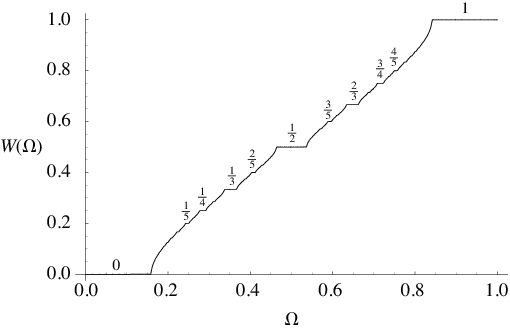
\includegraphics[width=0.6\textwidth]{media/Devil.png}
            \caption{A plot of $W(\Omega)$ grabbed from
            \url{http://mathworld.wolfram.com/DevilsStaircase.html}.\label{fig:19.devil}}
        \end{figure}

    \item The sum of the widths of the rational steps in the figure above tends
        to $0$ for $K \to 0$ and to unity as $K \to 1$. Interestingly, these
        rational steps are known as ``Arnold tongues.''
\end{itemize}

\subsection{$K = 1$}

\begin{itemize}
    \item At $K = 1$, the map develops an inflection point at $x=0$.

    \item The measure of $\Omega$ giving irrational $W$ is $0$, as the sum of
        the widths of the rational steps is $1$ from above. It turns out the set
        has fractal dimension $0.87$.

    \item Since passing through the inflection point yields chaos, and
        irrational winding number solutions tend to visit every point on the
        interval, irrational winding number solutions break down to chaos at
        $K=1$.

    \item Since rational winding number solutions visit a discrete number of
        points of the map, they tend not to break down to chaos.
\end{itemize}

\subsection{$K > 1$}

\begin{itemize}
    \item The Arnold tongues may overlap, which produces hysteresis.

    \item The map has a quadratic maximum, and similar to the quadratic map even
        periodic solutions can break down to chaos via period doubling cascades.
\end{itemize}

\clearpage

\section{Universal Onset of Chaos from a 2-torus}

We will adopt a similar approach to that used for the circle map for a
quasiperiodic torus, but the best way to examine the problem isn't to increase
$K$ for fixed $\Omega$, but rather to increas for fixed winding number $W$. This
makes the theory a bit more difficult, but let's sketch the argument here.

For any quasiperiodic orbit, we must examine irrational winding numbers. We will
formulate our plan of attack with a series of rational approximations, the
theory for which is founded in the theorem that any irrational number can be
uniquely written in a continued fraction expansion. Truncating this continued
fraction at the $n$th level gives the $n$th rational approximant $W_n$ to
irrational $W$.

Just a curious fact before we continue: define integers $(a_1, a_2,\dots)$ to be
the integers in the continued fraction
\begin{align}
    W &= \frac{1}{a_1 + \frac{1}{a_2 + \frac{1}{\dots}}},
\end{align}
then it turns out that all solutions to quadratic equations have periodic
rational expansion $(a_1, a_2,\dots)$. Moreover, the Golden mean
$\frac{\sqrt{5} - 1}{2}$ corresponds to $(1,1,\dots)$, which produces the
slowest converging rational expansion. The silver mean donetos $\sqrt{2} - 1$,
which corresponds to $(2,2,2\dots)$.

We will first motivate the discussion with some numerical results for the circle
map, then study the renormalization group theory for this system.

\subsection{Circle Map Results}

\begin{itemize}
    \item Define $G_n$ the $n$th rational approximation to the golden mean, then
        $\Omega_n(K)$ is the value of $\Omega$ for a given $K$ that produces
        winding number $G_n$. This results in the trajectory
        $f_{K,\Omega_n}^{F_{n+1}}$. We can then find that
        \begin{align}
            \lim_{n \to \infty}\Omega_n(K) &=
                \Omega_\infty(K) - c\tilde{\delta}^{-n}
        \end{align}
        where $\Omega_\infty(K)$ produces winding number $G$ the golden mean
        itself, and
        \begin{align}
            \tilde{\delta} &=
            \begin{cases}
                G^{-2} = 2.618\dots & K < 1\\
                2.8336\dots & K = 1
            \end{cases}
        \end{align}
        where the $K < 1$ case can be determined simply by looking at uniform
        rotation, but the $K = 1$ must be computed numerically.

    \item The distance $d_n$ from $x=0$ to the nearest other element of the
        $G_n$ cycle scales as
        \begin{align}
            \frac{d_n}{d_{n+1}} \to \tilde{\alpha}
        \end{align}
        with
        \begin{align}
            \tilde{\alpha} &=
            \begin{cases}
                -G^{-1} = -1.618\dots & K < 1\\
                -1.28857\dots & K = 1
            \end{cases}
        \end{align}

    \item Note that $\tilde{\delta}, \tilde{\alpha}$ are universal to all maps
        for a given winding number.
\end{itemize}

\subsection{Renormalization}

Since we notice that the point separation has some nice scaling structure, let's
renormalize the orbits. Define
\begin{align}
    \bar{f}^n(x) &= f^{F_{n+1}}(x) - F_n
\end{align}
and the scaled
\begin{align}
    \bar{f}_n(x) &= \tilde{\alpha}^n f^{F_{n+1}}(\tilde{\alpha}^{-n}x) - F_n.
\end{align}

These functions exhibit the property
\begin{align}
    \bar{f}^{n+1}(x) &= \bar{f}^n\left( \bar{f}^{n-1}(x) \right)
\end{align}

We now look for a fixed point structure, i.e.\ a function $\bar{f}^*$ satisfying
\begin{align}
    \bar{f}^*(x) &= \tilde{\alpha} \bar{f}^*\left(
        \tilde{\alpha}\bar{f}^*\left( \tilde{\alpha}^{-2}x \right)
    \right)
\end{align}

One such solution is $\bar{f}^*(x) = x + C$, which gives $\tilde{\alpha} =
-G^{-1}$. When $K=1$, the linear term disappears, and a second solution with the
numerical $\tilde{\alpha}$ appears. We can perform this analysis by linearizing
about the fixed point.

\clearpage

\section{Ruelle-Takens Theorem}

The Ruelle-Takens Theorem, later extended with Newhouse (henceforth referred to
as RTN), was initially misunderstood due to its highly mathematical language but
is still very useful. It concerns whether chaos arises from accumulation of
bifurcations or whether low-dimensional chaos is an additional route to chaos.
Its statement follows:
\begin{center}
    Let $v$ be a constant vector field on the torus $T^n = R^n/Z^n$. If $n \geq
    3$ then every $C^2$ neighborhood of $v$ contains a vector field $v'$ with a
    strange \emph{Axiom A} attractor. If $n \geq 4$ we may take $C^{\infty}$
    instead of $C^2$.
\end{center}

That's a mouthful. Can we clarify a bit?
\begin{itemize}
    \item For a set of ODEs $\rd{\vec{x}}{t} = \vec{v}(\vec{x})$, we call
        $\vec{v}(x)$ the vector field that generates the flow $\vec{x}(t)$.

    \item A constant vector field on an $n$-torus corresponds to uniform
        rotation in each of the $n$ directions, generally quasiperiodic.

    \item $C^2$ refers to twice differentiable, $C^\infty$ means
        smoothl/infinitely differentiable.

    \item An \emph{Axiom A} attractor is an attractor with many nice properties
        such as robustness under small parameter changes.
\end{itemize}

Thus, the RTN theorem says that it's possible to make certain arbitrarily small
perturbations to turn motion from an quasiperiodic $n$torus to chaotic for $n
\geq 3$. However, the chaotic motion remains \emph{on} the torus, and is robust
to further arbitrarily small perturbations. The ``every'' neighborhood refers to
the fact that all points in the vector field have such perturbations, but not
that a generic perturbation effects chaos. This was a stumbling point in early
use/interpretation of the theorem.

We do some numerical investigations of the theorem to illustrate precisely this
point, that a system that moves beyond linear dynamics is equally likely to
break down to period locked motion as to chaos.

\clearpage

\section{Mathematical Chaos}

\subsection{Definitions}

\begin{description}
    \item[Stable/Unstable Manifolds] In a given map $F(x)$ and a fixed point
        $x_f$, the stable manifold is the set of points such that $\abs{F^n(y) -
        F^n(x_f)} \to 0$ as $n \to \infty$, while the unstable manifold is the
        set of points such that $\abs{F^{-n}(y) - F^{-n}(x_f)} \to 0$ as $n \to
        \infty$.

        In a 2D map, the stable/unstable manifolds are 1D manifolds, where a
        manifold is a set that exhibits nice properties e.g.\ no fractal
        properties. A 1D manifold in particular must look locally like a single
        line everywhere (e.g.\ the letter A would not be a 1D manifold since the
        intersection points don't look like single lines but intersections).
        More generally, a manifold must at every point look ``like Euclidean
        space.''

    \item[Hyperbolic Invariant Sets] Hyperbolic invariant sets are
        generalizations of saddle points in multiple dimensions. For some point
        $x$ in a map $F$, we look at the linearized map about $x$, called the
        \emph{tangent space} $T_x$. An invariant set $\Sigma$ under $F$ is said
        to be hyperbolic if it decomposes into stable and unstable spaces $T_x =
        E^s \oplus E^u$ such that
        \begin{itemize}
            \item The splitting varies continuously with $x$.
            \item The action of the Jacobian about any $F^n(x)$ on any $v$ in
                the manifolds is bounded away from $0$, i.e.\ the exponetial
                growth/decayof the stable/unstable manifolds is bounded away
                from $0$.
        \end{itemize}

    \item[Axiom A attractor] These are attractors of differentiable maps that
        are hyperbolic and mixing. A mixing attractor means that for any two
        sets in the phase space
        \begin{align}
            \lim_{n \to \infty}\mu\left[ S_a \cap F^n(S_b) \right] &=
            \mu(S_a)\mu(S_b)
        \end{align}
        where $\mu$ is the measure of the attractor. In other words, points in
        the phase space are spread evenly over the attractor over time. Axiom A
        attractors are the nicest attractors and are structurally stable to
        small perturbations to the map.
\end{description}

Many physical attractors are non-hyperbolic b/c their stable/unstable manifolds
are tangent, and structural stability is in general hard to find. One example of
a map with an Axiom A attractor is the Ansov map
\begin{align}
    x_{n+1} &= x_n + y_n \mod 1\\
    y_{n+1} &= x_n + 2y_n \mod 1
\end{align}
since initial conditions fill the space with uniform measure. The Sinai map
\begin{align}
    x_{n+1} &= x_n + y_n + \delta \cos\left( 2\pi y_n \right)\mod 1\\
    y_{n+1} &= x_n + 2y_n \mod 1
\end{align}
is a small perturbation which therefore is also hyperbolic. However, dynamics
don't generally fill the map uniformly anymore, and we will explore this
next lecture.

\clearpage

\section{Predicting Chaos}

We want to be able to predict chaos, so we need to understand how homoclinic and
heteroclinic orbits behave under perturbation. We will develop these ideas from
sets that are not necessarily attractors, starting with the shift map.

The shift map is defined $x_{n+1} = 2x_n \pmod 1$. Consider our initial value as
an infinite decimal in binary, then the shift map serves simply to bitshift and
truncate the integer part. This exhibits the following properties
\begin{description}
    \item[Sensitivity to initial conditions] Two initial conditions arbitrarily
        close diverge after a sufficient number of iterations.

    \item[Symbolic dynamics] If we consider each value in a sequence of values
        generated by the map and round to $0,1$, we get a perfectly random
        sequence. The mapping of chaotic dynamics to random sequences is known
        as symbolic dynamics. A sequence of $0,1$s is a Bernoulli sequence.

    \item[Kolmogorov Entropy] Information is created at $1$ bit per iteration,
        thus the Kolmogorov entropy is $1$.

    \item[Most initial conditions are chaotic] All rational $x_0$ lead to
        periodic orbits, which is of measure zero; irrationals lead to chaotic
        orbits.
\end{description}

\subsection{Chaos in non-attractor sets: Smale Horseshoe}

We can define chaos as following: given any Bernoulli sequence, we can find an
initial state that reproduces exactly that sequence.

Let's consider this in the case of the Smale Horseshoe. The construction is as
follows:
\begin{itemize}
    \item Take a unit square and stretch it into a long vertical rectangle with
        width $1/\lambda$ and height such that two $1/\mu$-height sections at
        the top and bottom of the original unit square are now unit height.

    \item Map the images of these $1/\mu$-height sections (which are now unit
        height and $1/\lambda$ width) to the left and right of a new unit
        square.
\end{itemize}

We note that nothing with $y \in [1/\mu, 1-1/\mu]$ of the pre-image is mapped
into the image, and nothing with $x \in [1/\lambda, 1-1/\lambda/]$ has a
pre-image. Thus, with repeated iteration of this map, only a measure $0$ set of
the initial unit square survives, the invariant set.

We can denote each point with a $0, 1$ depending on which of the two slices it
lives in. Then, each point in the invariant set is denoted by an infinite
sequence of $0,1$s, and the effect of each iteration is to left-pop the sequence.
Since for any arbitrary sequence of $0,1$s, we can find a point in the invariant
set that generates this sequence, the Smale Horseshoe exhibits chaos.

\subsection{Homoclinic Tangles}

We introduced stable/unstable manifolds last section. Note that [un]stable
manifolds cannot intersect any other [un]stable manifolds, including itself,
since then that point will not have a unique inverse (or forward iteration of
the map). However, a stable manifold can intersect an unstable manifold, and if
the intersection is transverse rather than tangential, then the neighborhood of
the intersection can be shown to look like a Smale horseshoe (with all the
stretching/compressing dynamics at play\dots). This is called a homoclinic
tangle.

\subsection{Controlling Chaos}

There are a few chapters here that I don't feel like reading that talk about how
to control chaos. Since all chaotic attractors have unstable periodic orbits of
arbitrary period, it's possible to apply small perturbations to restore a
trajectory deviating from an unstable trajectory to keep it on. This goes into
some control theory.

It's also a cool way to compute gravitational slingshot-like problems: since the
systems are chaotic, it's possible to effect a large change in the trajectory
with an appropriately small perturbation. The formalism to do so is to grow the
trajectory backwards from the target and a stability zone, and forward from the
initial condition, find the minimum distance between these spheres and make the
appropriate perturbation.

\clearpage

\section{Hamiltonian Chaos}

The majority of Hamiltonian systems are not integrable, and most Hamiltonian
systems exhibit chaos. Since Hamiltonian systems preserve phase space, there can
be no attractors. Let's set out the basics of the discussion.

\subsection{Phase Space}

Phase space is described by $N$ position and momentum coordinates each, forming
a $2N$ phase space. The Hamiltonian satisfies the property
\begin{align}
    \rd{\vec{p}}{t} &= -\pd{H}{\vec{q}} & \rd{\vec{q}}{t} &= \pd{H}{\vec{p}}
\end{align}
where $H(\vec{p}, \vec{q}, t)$. Note that if $H$ has no explicit time dependence
then $\rd{H}{t} = 0$ is a constant that we call the energy. Hamiltonian dynamics
are volume preserving, i.e.
\begin{align}
    \vec{\nabla} \cdot \vec{V}_{ph} &= \pd{}{\vec{p}}\rd{\vec{p}}{t} +
        \pd{}{\vec{q}}\rd{\vec{q}}{t} = 0
\end{align}
or more strictly the symplectic property
\begin{align}
    \rd{}{t}\left( \delta \vec{p} \delta\pvec{q} -
        \delta \vec{q} \delta \pvec{p}\right) = 0
\end{align}
where $(\delta \vec{p}, \delta \vec{q})$ and its primed counter part are the two
separations between three infinitesimally separated orbits.

Canonical transformations are defined by a generating function
\begin{align}
    \pvec{q} &= \pd{S}{\pvec{p}}& \vec{p} &= \pd{S}{}\vec{q}
\end{align}
where $S(\pvec{p}, \vec{q}, t)$ is one possible choice of generating function.

For a $2N$-dimensional Hamiltonian, dynamics operate on a $2N-1$ subspace
constrained by the energy. Then, if we examine along a single constant plane
(e.g.\ maybe constant $q_i$) then we obtain a map. Moreover, thanks to the
Hamiltonian properties, we can show that the map is also symplectic. This means
that the eigenvalues governing displacement from a fixed point must come in
$(\lambda, 1/\lambda)$ pairs.

\subsection{Non-integrable systems}

An integrable Hamiltonian means that there are $N$ independent constants of
motion. We can start examining this by perturbing an integrable Hamiltonian
\begin{align}
    H &= H_0 + \epsilon H_1.
\end{align}

In general, $H$ is non-integrable for any $\epsilon > 0$. The motion under $H_0$
is an $n$torus with some frequency vector $\vec{\omega}$ at which the torus is
traversed (recall action-angle canonical transformations). What happens to these
trajectories as $\epsilon$ is increased?

For $2D$ tori (easiest to reason about since winding numbers only exist for
ratios of two frequencies), rational winding numbers break down for any
$\epsilon$, and irrational winding numbers break down depending on how close
they are to rationals (e.g.\ when we earlier talked about repeated fraction
expansions of irrational numbers, smaller numbers = ``more irrational.'').

The qualitative exploration of this behavior is in a lost set of lecture notes
\frownie.

\clearpage

\section{Quantum Chaos}

We explore what happens when we include $\hbar$ in chaotic classical
Hamiltonians. There should be some correspondence when $\hbar \to 0$ right?

We note that with a nonzero $\hbar$, the energy spectrum is no longer continuous
but discrete, and so the power spectrum cannot exhibit the broad bands
characteristic of chaos but is instead quasiperiodic, with frequencies
corresponding to the $E_n$. For instance, the energy dependent solutions look
something like
$\sum\limits_{n}^{} A_ne^{-i E_n t/\hbar}$.

The average splitting between energy levels can be estimated by phase space
volume: if we have a particle in a 2D box of dimensions $L$ and maximum energy
$E$, then there are of order $mEL^2/\hbar^2$ eigenstates, which gives an energy
splitting of $\hbar^2/mL^2$. Thus, in general, quantization should squelch
chaotic behavior since there's a maxiumum frequency!

\subsection{Energy Level Distribution}

It is difficult to predict the exact energy levels of quantum analogs to
classical chaotic systems given our poor characterization of the classical
motion, we probably can only make statistical predictions about the dynamics. We
choose $P(s)$ the probability distribution of $s$ the separation of adjacent
energy levels relative to the mean energy level spacing at that energy.

It turns out that $P(s)$ has functional form $\frac{\pi}{2}se^{-\pi s^2/4}$,
suggested by Wigner. This differs from what we would expect if the levels were
randomly distributed, which would produce Poissonian distributions.

It also turns out that the correct distribution can be produced by the
eigenvalues of random real, Hermitian matricies, with a distribution that turns
out to be simply Gaussian in each element $H_{jk}$. Real Hamiltonians are only
when time reversal is satisfied, and when it is broken, we can have just random
Hermitian matricies.

\clearpage

\appendix

\section{Revisiting Hamiltonian Chaos (borrowed from 106 notes)}

We will perform the entire discussion for only $N=1$, but since the Hamiltonian
and all of the operations are linear in the action or the angle, the
generalization should be obvious.

\subsection{Action-angle canonical transformation}

We start from the perspective of action-angle variables and canonical
transformations. An integrable system with $N$ degrees of freedom has $N$
constants of motion that can be chosen as action variables in action-angle
transformations. The motion of the system can then be thought of as on an
$N$-torus phase space, corresponding to the $N$ constants of motion.

To make the transformation to action-angle variables, consider the generating
function $S(I,q)$ satisfying
\begin{align}
    \theta &= \pd{S}{I} & p &= \pd{S}{q}\\
    H\left( \pd{S}{q}, q \right) &= H(I) = \text{constant}
\end{align}
such that the Hamiltonian is independent of $\theta$ the angle coordinate, which
idly ambles forward at a constant rate $\pd{H}{I}$. This formalism generalizes
naturally to multiple dimensioens.

\subsection{Perturbation theory of generating function}

Now we wish to add $H = H_0 + \epsilon H_1$ and see whether the new Hamiltonian
preserves the $N$-torus. If so, there must be another set of action-angle
variables $(\theta', I')$ for the new Hamiltonian. Let's construct a generating
function for the change of dynamical variables $(\theta, I) \to (\theta', I')$,
expressable as a power series
\begin{align}
    S(I', \theta) &= I'\theta + \epsilon S_1(I', \theta)
\end{align}
where the zeroth order term is simply the identity generating function. We plug
this into the Hamilton-Jacobi equation $H(I,\theta) = H'(I')$. This affects the
Hamiltonian as
\begin{align}
    H_0(I) + \epsilon\left[
        \omega_0(I) \cdot \pd{S_1}{\theta} + H_1(I,\theta)\right]
        + \mathcal{O}(\epsilon^2) &= H'(I')
\end{align}
where $\omega_0$ is just the zeroth order frequency. We must make the first
order terms cancel out.

We then leverage the fact that $S, S_1$ must both be periodic in $\theta$, since
$\theta$ is an angle coordinate (with period $2\pi$), and so we can express
$S_1, H_1$ in a Fourier series
\begin{align}
    H_1 &= \sum\limits_{m \neq 0}^{} H_{1,m}(I)e^{im\theta} &
    S_1 &= \sum\limits_{m \neq 0}^{} S_{1,m}(I)e^{im\theta}
\end{align}
which we can then substitute into the Hamilton-Jacobi equation to produce with
some small effort
\begin{align}
    S_{1,m} &= i\frac{H_{1,m}(I,\theta)}{m\omega}
\end{align}

For the multi-dimensional result, we replace $m\omega \to \vec{m} \cdot
\vec{\omega}$ and we obtain
\begin{align}
    S(\vec{I}, \vec{\theta}) &= \vec{I} \cdot \vec{\theta} + i\epsilon
        \sum\limits_{\vec{m} \neq 0}^{}\frac{H_{1,m}(\vec{I}, \vec{\theta})}
        {\vec{m} \cdot \vec{\omega}}e^{i\vec{m} \cdot \vec{\omega}}
\end{align}
and we obtain the expected result, that if the frequencies $\omega$ are such
that $\vec{m} \cdot \vec{\omega} = 0$ for any choice of $\vec{m}$ then the
perturbation theory diverges. Moereover, we see that the perturbation theory
term explodes inversely with ``how irrational'' the ratio between the
$\vec{\omega}$ are, since it dictates how small of a number $\vec{m} \cdot
\vec{\omega}$ can be for choices of $\vec{m}$.

We have thus proved a fraction of the Kolmogorov–Arnold–Moser (KAM) theorem. How
irrational winding numbers break down (they approach rational winding numbers
then break down) is a subject of another discussion, beyond my reach.
\end{document}
